\documentclass[a4paper,11pt,twoside]{scrartcl}
\usepackage[T1]{fontenc}
\usepackage{subcaption}
\usepackage[utf8]{inputenc}
\usepackage{ngerman, eucal, mathrsfs, amsfonts, bbm, amsmath, amssymb, stmaryrd,graphicx, array, geometry, color, wrapfig, float, hyperref, epstopdf,gensymb, subcaption, extarrows}
\geometry{left=25mm, right=15mm, bottom=25mm}
\setlength{\parindent}{0em} 
\setlength{\headheight}{0em} 
\title{Graphenalgorithmen\\ Blatt 7}
\author{Markus Vieth\and Christian Stricker}
\date{\today}
\usepackage{listings, textcomp}
\usepackage[usenames,dvipsnames,svgnames,table]{xcolor}


\definecolor{Code}{rgb}{0,0,0}
\definecolor{Keywords}{rgb}{0,0,255}
\definecolor{Strings}{rgb}{255,0,0}
\colorlet{Comments}{Green}
\colorlet{Numbers}{blue}

%%%%%%%%%%%
%Mache Integer farbig
%%%%%%%%%%%

\makeatletter

\newif\iffirstchar\firstchartrue
\newif\ifstartedbyadigit

\newcommand\processletter
{%
	\ifnum\lst@mode=\lst@Pmode%
	\iffirstchar%
	\global\startedbyadigitfalse%
	\fi
	\global\firstcharfalse%
	\fi
}

\newcommand\processdigit
{%
	\ifnum\lst@mode=\lst@Pmode%
	\iffirstchar%
	\global\startedbyadigittrue%
	\fi
	\global\firstcharfalse%
	\fi
}

\lst@AddToHook{Output}%
{%
	\ifstartedbyadigit%
	\def\lst@thestyle{\color{Numbers}}%
	\fi
	\global\firstchartrue%
	\global\startedbyadigitfalse%
}

\newtoks\jubo@toks
\jubo@toks={
	language=C,
	commentstyle=\color{Comments}\slshape,
	stringstyle=\color{Strings},
	keywordstyle={\color{Keywords}\bfseries},
	alsoletter=0123456789,
	SelectCharTable=%
}
\def\add@savedef#1#2{%
	\begingroup\lccode`?=#1\relax
	\lowercase{\endgroup
		\edef\@temp{%
			\noexpand\lst@DefSaveDef{\number#1}%
			\expandafter\noexpand\csname lsts@?\endcsname{%
				\expandafter\noexpand\csname lsts@?\endcsname\noexpand#2}%
		}}%
		\jubo@toks=\expandafter{\the\expandafter\jubo@toks\@temp}%
	}
	\count@=`0
	\loop
	\add@savedef\count@\processdigit
	\ifnum\count@<`9
	\advance\count@\@ne
	\repeat
	\count@=`A
	\loop
	\add@savedef\count@\processletter
	\ifnum\count@<`Z
	\advance\count@\@ne
	\repeat
	\count@=`a
	\loop
	\add@savedef\count@\processletter
	\ifnum\count@<`z
	\advance\count@\@ne
	\repeat
	%\showthe\jubo@toks % for debugging
	\begingroup\edef\x{\endgroup
		\noexpand\lstdefinestyle{pseudo}{\the\jubo@toks}
	}\x
	
	\makeatother
%%%%%%%%%%
%Ende
%%%%%%%%%%



\lstset{
	literate={ö}{{\"o}}1
	{ä}{{\"a}}1
	{ü}{{\"u}}1
	{ß}{{\ss}}1
	{/pi}{{$\Pi$}}1
	{/inf}{{$\infty$}}1
	{/eIn}{{$\in$}}1
	{/cup}{{$\cup$}}1
	{/leer}{{$\emptyset$}}1
	{<=}{{$\leq$}}1
	{>=}{{$\geq$}}1
	{→}{{$\rightarrow$}}1
	{⊈}{{$\not\subseteq$}}1
	{⊆}{{$\subseteq$}}1
	{∉}{{$\notin$}}1
	{∈}{{$\in$}}1
	{⇒}{{$\Rightarrow$}}1
	{∪}{{$\cup$}}1
	{α}{{$\alpha$}}1
	{∅}{{$\emptyset$}}1	
}


\lstset{
	numberstyle=\tiny,
	stepnumber=1,
	numbersep=10pt,
	xleftmargin=15pt,
	breaklines=true,
	numberblanklines=false,
	showstringspaces=false,
	flexiblecolumns=true,
	mathescape=true,
	tabsize=4,
	captionpos=b,
	numbers=left,
	commentstyle=\color{Green},
	numberstyle=\color{gray},
	keywordstyle=\color{blue} \textbf,%otherkeywords={xdata},
	keywords=[2]{xdata},
	keywordstyle=[2]\color{red}\textbf,
	identifierstyle=\color{black},
	stringstyle=\color{red}\ttfamily,
	basicstyle = \ttfamily \color{black} \footnotesize,
	inputencoding=utf8,
	emph=[1]%
	{%
		infinity,
	}, 
	emphstyle=[1]{\color{blue}},
	emph=[2]%
	{%
		forall,
		while,
		if,
		else,
		for,
		return,
		new,
		NULL,
		null,
		int, 
		double, 
		float,
		class,
		void,
		false, 
		true,
		FALSE,
		TRUE,
	}, 
	emphstyle=[2]{\color{Magenta}},
	emph=[3]{b0, b1, n0, n1},
	emphstyle=[3]{\color{black}}
}
\usepackage{float}
\usepackage[section]{placeins}
\usepackage{epstopdf}
\usepackage{wrapfig}
\usepackage{caption}
\usepackage{subcaption}
\usepackage{graphicx}
\usepackage{pgfplots}
\usetikzlibrary{plotmarks}
\usetikzlibrary{patterns}
\usetikzlibrary{decorations.pathmorphing}
\newcommand{\coloredcircled}[3][black]{{\large \Large\color{#2}\textcircled {{\small\color{#1}#3}}}}% Circlecolor, Textcolor, text
\newcommand{\ddvec}[2]{\begin{pmatrix}#1\\#2\end{pmatrix}}
\newcommand{\dddvec}[3]{\begin{pmatrix}#1\\#2\\#3\end{pmatrix}}
\newcommand{\longvec}[1]{\overset{\longrightarrow}{#1}}
\newcommand{\eunorm}[1]{\left\lVert#1\right\rVert_2}
\newcommand{\scalar}[2]{\left<#1,#2\right>}\newcommand{\cor}[1]{\textcolor{red}{\textit{#1}}}
\newcommand{\qed}{%
	\begin{flushright}
		q.e.d.
	\end{flushright}%
	}
\newcommand*\circled[1]{%
	\tikz[baseline=(char.base)]\node[shape=circle,draw,inner sep=0.2pt,font=\tiny,minimum size=8pt] (char) {#1};}
\renewcommand\thefootnote{\protect\circled{\arabic{footnote}}}
\begin{document}
\maketitle
\cleardoublepage
\pagestyle{myheadings}
\markboth{Markus Vieth, Christian Stricker}{Markus Vieth, Christian Stricker}

\newpage
\section{Aufgabe 1: FPT Vertex-Cover (10 P)}
\subsection{Vorüberlegung}
Aus $d(v) \leq 2$ folgt, dass der Graph nur aus Einzelknoten mit $d(v) = 0$, Strecken aus 2 Knoten mit $d(v) = 1$ und beliebig vielen Zwichenknoten mit $d(v) = 2$ sowie aus Zyklen in denen für alle Knoten gilt $d(v) = 2$.\\
Offensichtlich gilt, wir können alle Knoten mit $d(v) = 0$ ohne Schaden löschen. Für Pfade und Zykel wird eine Fallunterscheidung gemacht:
\subsubsection{Pfad mit gerader Knotenanzahl}
\begin{figure}[H]
	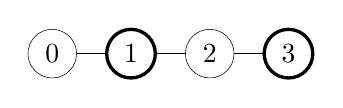
\begin{tikzpicture}
	\node[draw, circle, very thin] at (0,0) (0){0}; 
	\node[draw, circle, very thick] at (1,0) (1){1}; 
	\node[draw, circle, very thin] at (2,0) (2){2}; 
	\node[draw, circle, very thick] at (3,0) (3){3}; 
	\draw (0)-- (1)--(2)--(3);
	\end{tikzpicture}
\end{figure}
Es reicht von einer Seite anfangend jeden 2. Knoten ins Set aufzunehmen, angefangen mit dem zweitem. Durch Induktion lässt sich zeigen, dass diese Wahl immer minimal ist.
\subsubsection{Pfad mit ungerader Knotenanzahl}
\begin{figure}[H]
	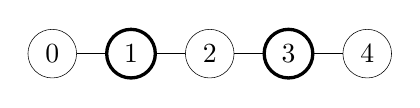
\begin{tikzpicture}
	\node[draw, circle, very thin] at (0,0) (0){0}; 
	\node[draw, circle, very thick] at (1,0) (1){1}; 
	\node[draw, circle, very thin] at (2,0) (2){2}; 
	\node[draw, circle, very thick] at (3,0) (3){3}; 
	\node[draw, circle, very thin] at (4,0) (4){4}; 
	\draw (0)-- (1)--(2)--(3)--(4);
	\end{tikzpicture}
\end{figure}
Es reicht von einer Seite anfangend jeden 2. Knoten ins Set aufzunehmen, angefangen mit dem zweitem. Durch Induktion lässt sich zeigen, dass diese Wahl immer minimal ist.
\subsubsection{Zykel mit gerader Knotenanzahl}
\begin{figure}[H]
	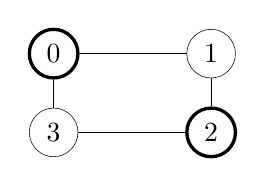
\begin{tikzpicture}
	\node[draw, circle, very thick] at (-1,1) (0){0}; 
	\node[draw, circle, very thin] at (1,1) (1){1}; 
	\node[draw, circle, very thick] at (1,0) (2){2}; 
	\node[draw, circle, very thin] at (-1,0) (3){3}; 
	\draw (0)-- (1)--(2)--(3)--(0);
	\end{tikzpicture}
\end{figure}
Es reicht von einem Knoten anfangend jeden 2. Knoten ins Set aufzunehmen, angefangen mit dem ersten. Durch Induktion lässt sich zeigen, dass diese Wahl immer minimal ist.
\subsubsection{Zykel mit ungerader Knotenanzahl}
\begin{figure}[H]
	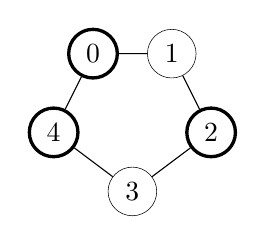
\begin{tikzpicture}
	\node[draw, circle, very thick] at (-.5,1) (0){0}; 
	\node[draw, circle, very thin] at (.5,1) (1){1}; 
	\node[draw, circle, very thick] at (1,0) (2){2}; 
	\node[draw, circle, very thin] at (0,-.75) (3){3}; 
	\node[draw, circle, very thick] at (-1,0) (4){4}; 
	\draw (0)-- (1)--(2)--(3)--(4)--(0);
	\end{tikzpicture}
\end{figure}
Es reicht von einer Seite anfangend jeden 2. Knoten ins Set aufzunehmen, angefangen mit dem ersten. Durch Induktion lässt sich zeigen, dass diese Wahl immer minimal ist.
\subsection{Pseudocode}
\begin{lstlisting}[language=Java]
Knoten[] findVertexCover($G=(V,E)$) {
	Knoten[] result;
	zuBesuchen = V;
	for(Knoten v in zuBesuchen) {  // Laufzeit in $O(n)$
		// Lösche alle Knoten vom Grad 0
		if(v.grad == 0) {
			zuBesuchen.remove(v);   // Bei geeigneter Datenstruktur (z.B. Hashing) $O(1)$
			continue;
		}
		// Bei Knoten vom Grad 1, suche Pfad ab und füge jeden 2. Knoten dem Ergebniss hinzu
		if(v.grad == 1) {
			boolean second = false;
			zuBesuchen.remove(v);   // Bei geeigneter Datenstruktur (z.B. Hashing) $O(1)$
			prev = NULL;
			while(v.hasNext(prev)) { // Laufzeit in $O(n)$
				second = !second;
				v = v.next(prev);  // $O(1)$
				zuBesuchen.remove(v);   // Bei geeigneter Datenstruktur (z.B. Hashing) $O(1)$
				if(second)
					result += [v];   // $O(1)$
			}
			continue;
		}
	} 
	// Da keine Knoten mehr vom Grad < 2 da sind, müssen alle anderen Knoten Zykel bilden
	for(Knoten v in zuBesuchen) { // Laufzeit in $O(n)$
		boolean second = false;
		zuBesuchen.remove(v);  // Bei geeigneter Datenstruktur (z.B. Hashing) $O(1)$
		result += [v];   // $O(1)$
		prev = NULL;
		first = v;
		while(v.next(prev) != first) { // Laufzeit in $O(n)$
			second = !second;
			v = v.next(prev);   // $O(1)$
			zuBesuchen.remove(v);   // Bei geeigneter Datenstruktur (z.B. Hashing) $O(1)$
				if(!second)
					result += [v];   // $O(1)$
			}
		}
	}
	return res;
}

class Knoten {
	// Liste benachtbarter Knoten
	Knoten[] nachbarn;

	int grad() { // $O(1)$
		return nachbarn.size();
	}

	// return nächst besten Nachbarn ungleich prev
	Knoten next(Knoten prev) { // $O(1)$
		if(prev != NULL && prev == nachbarn[0])
			return nachbarn[1];
		return nachbarn[0];
	}

	// wenn prev = null, hat dieser Knoten einen Nachbarn? sonst: Hat dieser Knoten einen Nachbarn ungleich prev?
	boolean hasNext(Knoten prev) { // $O(1)$
	if(prev == NULL)
		return this.grad > 0;
	boolean res = false;
	for(Knoten v in this.nachbarn)
		res |= (v == prev);  // Hier ist ein Fehler
		return res;
	}
}
\end{lstlisting}
$\Rightarrow$ Laufzeit in $O(n) * O(n) + O(n) * O(n) = O(n^2)$ und somit in polynomialer Zeit
\qed
\section{Aufgabe 2: FPT Pathfind (10 P)}
\subsection{$k \leq d$ }
\subsection{Pseudocode}
\begin{lstlisting}[language=Java]
Knoten[] findKPath(G,k) {
	Knoten[] result;
	if (k $\leq$ G.d ) {
		Knoten v = V[0];
		result += [v];
		v.setMarked(true);
		while(result.size < k) { // $O(k)$
			v = v.nextUnmarked(); // $O(d) \in O(n)$
			result += [v];
			v.setMarked(true);
		}
	} // $O(kn)$
	else 
	{
		// siehe Text
	}
}

class Knoten {
	// Liste benachtbarter Knoten
	Knoten[] nachbarn;
	boolean marked = false;
	
	void setMarked(boolean marked) {
		this.merked = marked;
	}

	// return nächst besten Nachbarn ungleich prev
	Knoten nextUnmarked() { // $O(d)$
		for(Knoten v in nachbarn)
			if(!v.marked)
				return v;
		return NULL;
	}
}
\end{lstlisting}
\subsection{$k > d$}
Parallel zur Vorlesung nutzen wir eine Tabelle und dynamische Programmierung:\\
Wir speichern in der Zelle $T[i,j]$ alle erlaubten Sequenzen der Länge $i$ startend beim Knoten $v_j$. Die erste Zeile beinhaltet somit $T[0,j] = \emptyset$, die zweite Zeile $T[1,j] = \{ v_j \}$. Im weiteren nehmen wir alle Pfade in die Zelle auf, für die gilt, dass sie aus $[v_j] + P$ bestehen, mit $P \in T[i-1,\ell]$ mit $\ell \neq j$. Machen wir das über alle Möglichkeiten ergibt sich als Formel:
\[ T[i,j] = \bigcup_{v_\ell | \{v_j,v_\ell\} \in E } \left\{ [v_j] + P | P \in T[i-1, \ell] \land v_j \notin P \right\} \]
Weiter gilt, dass ein Knoten $v_j$ genau $d$ Nachbarn hat, die in der obigen Vereinigung beachtet werden und das $i$ bis $k$ läuft. Für jede Zellen müssen maximal $d$ Werte betrachtet werden. Parallel zur Vorlesung gilt somit eine Tabellengröße von $d^k \cdot n$ und eine Laufzeit von $O(k^k \cdot n)$
\section{Aufgabe 3: FPT Independent-Set (10 P)}
\subsection{Vorüberlegung}
Für planare Graphen gilt nach dem Eulerschen Polyedersatz:
\[ |V| - |E| + |F| = 2 \]
Mit $F$ der Menge aller Oberflächen im Graphen die durch die Kanten des Graphen abgegrenzt sind. 
Dabei stellen wir uns vor, dass der betrachtet Ausschnitt oben und unten, sowie links und rechts verbunden sind und so dass die Fläche außerhalb des Graphen ebenfalls eine Oberfläche bildet. Da unser Graph einfach ist, wird jede Oberfläche von mindestens 3 Kanten aufgespannt (\textcircled{\small 2}). Weiter liegt eine Kante auf jeden Fall zwischen nicht mehr als 2 Oberflächen (\textcircled{\small 1}). Somit gilt:
\[ |F| \leq 2|E|\footnote{\textcircled{\tiny1}} \land 3|F| \leq |E|\footnote{\textcircled{\tiny2}} \]
\[ \Rightarrow |F| \leq  3|F| \leq |E| \leq 2|E| \]
\[ \Rightarrow 3|F| \leq 2|E| \]
\[ \Rightarrow |V| - |E| + \frac{2}{3}|E| \geq 2 \]
\[ \Leftrightarrow 3|V| - 6 \geq |E| \]
Für den durchschnittlichen Grad eine Knoten gilt dann:
\[ \frac{2*|E|}{|V|} \leq \frac{2(3*|V|-6)}{|V|} = 6 * \frac{|V| -2}{|V|} \leq 6 \]
Das Löschen eines Knoten in einem planaren Graphen ergibt wieder einen planaren Graphen.\\
So können wir immer an einem Knoten mit Grad 5 verzweigen, indem man einen der 6 Knoten zur Lösungsmenge hinzunimmt. Die Laufzeit beträgt somit $O(6^k\cdot poly(n))$.
\end{document}